\begin{titlepage}

    \centering

    \vspace*{\fill}

    {\LARGE\bfseries State Supreme Court Selection Mechanisms and Dissent\par}

    \vspace{1.5cm}

    {\large Alexandria Nagy\par}

    \vspace{0.5cm}

    {\large \today\par}

    \vspace*{\fill}

\end{titlepage}

\newpage

\subsection{Abstract}\label{abstract}

The present study examines the extent to which state supreme court
selection mechanisms shape judicial opinion-writing behavior and
reassesses dissent rates as a proxy for judicial independence. A
mixed-methods design combines synthetic control analysis of transitions
in selection mechanisms (2012--2024) with computational text analysis of
2.6 million opinions from all 50 state supreme courts (1970--2019).
Synthetic control estimates of shifts between partisan and nonpartisan
elections on the North Carolina Supreme Court reveal substantial
measurement sensitivity, covariate imbalance, and counterfactual
instability, yielding no reliable evidence that electoral reform
systematically alters dissent frequency and raising concerns about
dissent rates as a valid or reproducible measure of independence.
Textual analysis employs a Wordscores framework anchored in PAJID-based
seed dictionaries and expanded through Word2Vec embeddings to produce
rhetoric scores reflecting the balance of ideological and conventional
language in each opinion. Although pooled models show no statistically
significant differences in rhetoric scores across selection regimes,
event studies reveal directionally consistent rhetorical shifts
following institutional change, suggesting that linguistic content is a
more behaviorally sensitive indicator of institutional effects than
dissent frequency.

\subsection{Introduction}\label{introduction}

The United States is undergoing a profound transformation in its
judicial landscape. In a period marked by rising polarization and a more
openly majoritarian conservative constitutional order, the Supreme Court
of the United States has delegated responsibility for resolving many
contentious national issues to the states by narrowing federal oversight
in areas such as campaign finance, partisan gerrymandering, abortion,
and voting rights. As the stakes of state-level adjudication have
increased, the expected policy payoff of controlling state supreme
courts has risen as well. State legislatures and partisan actors have
responded by restructuring judicial selection systems to allow for
greater direct political influence, most prominently by replacing
nonpartisan judicial elections with explicitly partisan contests through
the inclusion of party affiliations on ballots. In 2025, Montana's
legislature advanced five proposals to introduce partisan judicial
contests.\footnote{Constance Van Kley, {``The {Montana Legislature}'s
  {Partisan Attack} on {Judicial Independence},''} in \emph{State Court
  Report}, 2025,
  \url{https://statecourtreport.org/our-work/analysis-opinion/montana-legislatures-partisan-attack-judicial-independence}.}
Although these measures were ultimately defeated in Montana, comparable
reforms have succeeded elsewhere. Ohio enacted Senate Bill 80 in 2021;
North Carolina passed Session Law 2016-125 in 2016; West Virginia
adopted Senate Bill 521 in 2025.\footnote{See Ohio S.B. 80 (2021); N.C.
  Sess. Law 2016-125 (2016); W. Va. S.B. 521 (2025).} Each of these laws
requires candidates to list party affiliation on both primary and
general election ballots, thereby formalizing partisanship in state
supreme court elections.

Against this backdrop, scholars remain divided over whether the shift
toward partisan judicial selection effectively balances judicial
independence and accountability, two principles that are inherently in
tension.\footnote{See Melinda Gann Hall, {``State {Supreme Courts} in
  {American Democracy}: {Probing} the {Myths} of {Judicial Reform},''}
  \emph{The American Political Science Review} 95, no. 2 (2001):
  315--30, \url{https://www.jstor.org/stable/3118123} for an overview of
  the scholars involved in this debate} Judicial independence allows
courts to decide cases based on law and free from external pressures,
while accountability requires them to remain responsive to public values
and societal needs. Reform advocates tend to argue that partisan
elections place too much emphasis on party loyalty and electoral
considerations, undermining independence and risking decisions driven
more by politics than by legal reasoning. They generally favor
nonpartisan elections or merit-based retention systems, such as the
Missouri Plan, to prioritize professional qualifications and preserve
judicial autonomy. In contrast, opponents of reform contend that
partisan elections enhance democratic accountability without necessarily
eroding independence, as electoral competition incentivizes judges to
remain attentive to voter concerns. This debate highlights how different
selection mechanisms structure judicial incentives and shape the
potential for systematic bias in judicial decision-making.

This study extends scholarship on judicial independence in state supreme
courts by examining the institutional shift from nonpartisan to partisan
judicial elections. Prior research has employed a range of empirical
strategies to estimate how selection mechanisms influence dissent rates,
which are frequently used as a behavioral proxy for judicial
independence.\footnote{Bradley C. Canon and Dean Jaros, {``External
  {Variables}, {Institutional Structure} \& {Dissent} on {State Supreme
  Courts},''} \emph{Polity} 3, no. 2 (1970): 175--200,
  \url{https://doi.org/10.2307/3233984}; Matthew E. K. Hall and Jason
  Harold Windett, {``New {Data} on {State Supreme Court Cases},''}
  \emph{State Politics \& Policy Quarterly} 13, no. 4 (2013): 427--45,
  \url{https://www.jstor.org/stable/24710959}; Kristen M. Renberg,
  {``The {Impact} of {Retention Systems} on {Judicial Behavior}: A
  {Synthetic Controls Analysis} of {State Supreme Courts},''} \emph{The
  Justice System Journal} 41, no. 4 (2020): 292--312,
  \url{https://www.jstor.org/stable/27224753}.} These approaches include
manual data collection, automated web scraping using Python, and
quasi-experimental techniques such as the synthetic control method
(SCM). Despite these advances, dissent rates remain an imperfect measure
and are vulnerable to concerns about data completeness, reproducibility,
and construct validity. As language modeling techniques advance,
computational textual analysis of judicial opinions offers a more
complete understanding of judicial behavior than dissent rates alone. By
distinguishing ideological from conventional language, this approach
provides insight into how institutional design shapes judicial rhetoric.
This study therefore evaluates whether partisan and nonpartisan
selection mechanisms influence patterns of opinion-writing and considers
what these differences imply for the measurement of judicial
independence in state supreme courts.

\subsection{Literature Review}\label{literature-review}

There are two main strands of research on the impacts of judicial
selection mechanisms on independence. The first uses dissent rates as a
behavioral proxy: a justice's decision to write a dissent reflects a
willingness to challenge the majority opinion, advance alternative legal
interpretations, and resist political or institutional
pressures.\footnote{Renberg, {``The {Impact} of {Retention Systems} on
  {Judicial Behavior}.''}} The most directly relevant body of this
scholarship examines how selection mechanisms shape dissent rates. Brace
and Hall find that appointed judges tend to promote consensus, while
elected judges are associated with higher dissent rates.\footnote{Paul
  Brace and Melinda Gann Hall, {``Neo-{Institutionalism} and {Dissent}
  in {State Supreme Courts},''} \emph{The Journal of Politics} 52, no. 1
  (1990): 54--70, \url{https://doi.org/10.2307/2131419}.} Jaros and
Canon report the same pattern, finding that popularly elected courts
dissent more frequently than appointed ones.\footnote{Canon and Jaros,
  {``External {Variables}, {Institutional Structure} \& {Dissent} on
  {State Supreme Courts}.''}} Hall and Windett offer a systematic
comparison across four selection systems, including gubernatorial or
legislative appointment, the Missouri Plan, nonpartisan elections, and
partisan elections. They find that appointed and Missouri Plan courts
exhibit stable, low dissent rates, which the authors attribute to longer
tenures, greater professionalization, and insulation from electoral
pressure.\footnote{Matthew E. K. Hall and Jason Harold Windett,
  {``Discouraging {Dissent}: {The Chief Judge}'s {Influence} in {State
  Supreme Courts},''} \emph{American Politics Research} 44, no. 4
  (2016): 682--709, \url{https://doi.org/10.1177/1532673X16640743}.}
Nonpartisan election courts dissent at higher rates than Missouri Plan
states, suggesting that electoral incentives shape judicial behavior
even without party labels on the ballot. Lastly, partisan election
courts show the most pronounced and unstable patterns, which the authors
attribute to potential reelection pressures. Renberg extends this line
of inquiry using synthetic controls, finding that removing partisan
labels from ballots increases dissenting opinions. This suggests that
justices strategically moderate dissent under partisan constraints and
use dissent more freely when party identifiers are removed.\footnote{Renberg,
  {``The {Impact} of {Retention Systems} on {Judicial Behavior}.''}}

A credible analysis of selection mechanism effects must also account for
confounding factors at the interpersonal, environmental, and
institutional levels. At the interpersonal level, Jaros and Canon
identify strong chief justice leadership, high social integration, and a
norm of unanimity as forces that cultivate consensus.\footnote{Canon and
  Jaros, {``External {Variables}, {Institutional Structure} \& {Dissent}
  on {State Supreme Courts}.''}} Hall and Windett show that chief
justices actively discourage dissent to foster collegiality, reinforce
precedent, and bolster public confidence, as dissent imposes costs on
colleagues, risks weakening precedent, and encourages future
appeals.\footnote{Hall and Windett, {``New {Data} on {State Supreme
  Court Cases}.''}} Dissent rates are lower on courts where the chief
holds greater formal powers and members have fewer institutional
resources; abundant resources undermine the chief's authority and
encourage dissent. Epstein, Landes, and Posner add that judges may
suppress dissent through what they term dissent aversion, though this
tendency weakens as ideological divisions widen and panel sizes
grow.\footnote{Lee Epstein et al., {``Why ({And When}) {Judges Dissent}:
  {A Theoretical And Empirical Analysis},''} \emph{Journal of Legal
  Analysis} 3, no. 1 (2011): 101--37,
  \url{https://doi.org/10.1093/jla/3.1.101}.}

At the environmental level, Brace and Hall find that higher
urbanization, greater political competition, and increased state
spending are each associated with elevated dissent rates.\footnote{Brace
  and Hall, {``Neo-{Institutionalism} and {Dissent} in {State Supreme
  Courts}.''}} Epstein, Landes, and Posner further show that
ideologically divergent panels dissent more frequently, and that courts
operating in more heterogeneous and competitive political contexts are
structurally more prone to disagreement.\footnote{Epstein et al., {``Why
  ({And When}) {Judges Dissent}.''}} At the institutional level, Brace
and Hall find that court structures account for roughly six times more
explanatory power than environmental variables.\footnote{Brace and Hall,
  {``Neo-{Institutionalism} and {Dissent} in {State Supreme Courts}.''}}
Beyond selection mechanism, the presence of intermediate appellate
courts increases dissent by filtering routine cases and leaving higher
courts to resolve more complex and contested disputes. Random opinion
assignment promotes dissent by limiting the chief justice's ability to
use discretionary assignments as rewards or sanctions, while conference
procedures that emphasize seniority encourage consensus by creating
incentives against open disagreement. Jaros and Canon confirm that
dissent rises with court size and falls with longer judicial
terms.\footnote{Canon and Jaros, {``External {Variables}, {Institutional
  Structure} \& {Dissent} on {State Supreme Courts}.''}}

Within this strand of the scholarship, an important gap remains. The
existing literature on selection mechanism effects and judicial behavior
has examined transitions in one primary direction: Renberg's synthetic
control analysis estimates the effect of moving from partisan to
nonpartisan elections on dissenting behavior.\footnote{Renberg, {``The
  {Impact} of {Retention Systems} on {Judicial Behavior}.''}} The
reverse transition, from nonpartisan to partisan elections, has received
comparatively little scholarly attention. This leaves open the question
of whether the behavioral effects of adding partisan labels to the
ballot are symmetric with those of removing them. The present study
addresses this gap directly by applying a synthetic control design to
the North Carolina Supreme Court, which experiences a transition from
nonpartisan to partisan judicial elections effective in 2018.

Renberg's study models counterfactual courts that represent the outcome
of dissent rates on the Arkansas, Tennessee, and Mississippi's state
supreme courts had there never been an electoral reform from partisan to
nonpartisan elections. Renberg finds that dissent rates on these courts
icreased, attributing this result to reduced partisan electoral
pressures that may otherwise constrain judicial expressions of
disagreement.

Scholarship examining dissent rates on state supreme courts faces two
primary challenges. The first is data availability. The FAIR principles
emphasize that scientific data should be findable, accessible,
interoperable, and reusable, with persistent identifiers, standardized
retrieval protocols, shared formats, and clear documentation of
provenance and licensing.\footnote{{Mark D. Wilkinson et al.}, {``The
  {FAIR Guiding Principles} for Scientific Data Management and
  Stewardship,''} \emph{Scientific Data} 3, no. 1 (2016): 160018,
  \url{https://doi.org/10.1038/sdata.2016.18}.} In practice, data on
dissent rates remain sparse, inaccessible, and difficult to replicate.
The State Supreme Court Data Project covers only four years
(1995--1998);\footnote{Paul Brace and Melinda Gann Hall, \emph{State
  {Supreme Court Data Project}}, n.d., accessed February 22, 2026,
  \href{https://www.ruf.rice.edu//textasciitilde\%20pbrace/statecourt/}{https://www.ruf.rice.edu/\textbackslash textasciitilde
  pbrace/statecourt/}.} Hall and Windett's data are inaccessible, and
their Python code relies on web scraping prohibited by
LexisNexis;\footnote{Hall and Windett, {``New {Data} on {State Supreme
  Court Cases}.''}} LexisNexis provides comprehensive coverage but its
proprietary structure limits transparency for researchers without
bulk-access subscriptions; and CourtListener, while open source, offers
substantially less complete coverage. These limitations prevent
independent verification and constrain cumulative knowledge on judicial
opinion writing and dissent rates.

The second challenge is reproducibility. Rather than presenting
numerical data, Renberg relies on graphical depictions with unclear
measurement conventions.\footnote{Renberg, {``The {Impact} of {Retention
  Systems} on {Judicial Behavior}.''}} Multiple strategies were
implemented to replicate the implied rates using CourtListener and
LexisNexis.\footnote{In CourtListener, searches were restricted by court
  and refined with advanced opinion-type operators, including
  combined-opinion, unanimous-opinion, lead-opinion, plurality-opinion,
  concurrence-opinion, in-part-opinion, dissent, addendum, remittitur,
  rehearing, on-the-merits, and on-motion-to-strike. LexisNexis searches
  employed the OpinionBy and DissentBy fields as well as the ``find by
  source'' function.} Replication also followed Hall and Windett's
method of dissent rate data collection.\footnote{Hall and Windett,
  {``New {Data} on {State Supreme Court Cases}.''}}\footnote{First, all
  justices serving on each court between 1995 and 2010 were queried
  using LexisNexis OpinionBy and DissentBy fields. Second, because Hall
  and Windett focus on ``cases in which a state supreme court rendered a
  final judgment with a full written opinion,'' queries excluded entries
  containing terms such as ``dismiss!,'' ``petition for review,'' and
  ``motion for,'' using AND NOT operators to restrict the dataset to
  full merits decisions.} Across databases and query configurations,
estimated dissent rates did not align with Renberg's graphs or Hall and
Windett's reported figures (see Table
\ref{tab:dissent_rates_replication}). Moreover, variation across query
constructions was substantial, indicating that dissent rate estimates
are highly contingent on operational definitions and database filters.
Without detailed documentation of coding rules, inclusion criteria, and
database parameters, baseline dissent rates cannot be independently
verified.

While dissent rates and voting records provide quantitative measures of
disagreement on the bench, they offer limited insight into the
underlying substance of judicial reasoning. A deeper examination of the
language judges choose when crafting opinions provides a richer
understanding of the ideological considerations at play that might be
missed by relying solely on quantitative behavioral measures (Bailey and
Maltzman, 2011; Hinkle, 2015; Songer and Lindquist, 1996). Computational
textual analysis has accordingly emerged as a powerful methodological
tool for examining the content of judicial opinions, with recent
advances in natural language processing and machine learning enabling
systematic analysis of how judges signal their ideological positions and
respond to external pressures. As Fischman and Law (2009) have argued, a
more complete conception of judicial ideology must grapple with how
judges think about the law, not just how they vote on cases. Similarly,
Hinkle (2015) and Songer and Lindquist (1996) have demonstrated that a
justice's values shape not only the direction of their votes, but also
the content and character of their written opinions, including which
precedents they recognize, how they frame legal standards, and how
broadly or narrowly they interpret statutory and constitutional
provisions. The intellectual premise underlying this approach is
articulated clearly by Truscott and Romano (2025), who observe that
terminology is an expression of language and language is an expression
of ideology. For example, the terms ``healthcare provider'' and
``abortionist'' both reference the same category of medical
professional, yet they carry dramatically different ideological
valences.

The motivation for text-based measurement is partly a critique of
existing vote-based approaches. Measures such as the widely used
Martin-Quinn scores, which rely on dynamic Bayesian estimation of ideal
points from observed voting patterns, are powerful and reliable.
However, although they offer insight into whether a justice voted
liberally or conservatively on a given case, these scores cannot
illuminate why or reveal the full texture of how ideological commitments
shape legal reasoning (Romano and Curry, 2019). It is also worth noting
that Martin-Quinn scores are developed for U.S. Supreme Court justices
specifically and do not extend to a comprehensive, widely-cited database
of state supreme court ideology.

Three foundational scaling approaches have been particularly influential
for text-based measurements of ideology. First, Wordscores is a
reference-document method that estimates the positions of new texts by
comparing their word frequencies to those of texts whose positions are
already known (Laver, Benoit, and Garry, 2003). Wordscores established
the foundational premise that lexical variation across documents encodes
positional information recoverable through computational analysis.
Second, Wordfish is an unsupervised scaling model that estimates actor
positions from word frequencies without requiring reference documents,
using a Poisson distribution to model word counts as a function of an
actor's underlying ideological position on a latent dimension (Slapin
and Proksch, 2008). Third, Wordshoal is a hierarchical extension of
Wordfish that addresses single scaling dimension limitations of
Wordfish, applying word-position associations learned in one domain
uniformly across all others (Lauderdale and Herzog, 2016). Wordshoal
implements a two-stage hierarchical strategy: first applying a Wordfish
model within each debate or case to recover local positional estimates,
then aggregating these into a global score by weighting each debate
according to how strongly its local dimension aligns with the common
latent dimension. Validated in the context of the U.S. House of
Representatives, Wordshoal produced highly reliable estimates of member
ideology from floor speeches, making it a natural candidate for
adaptation to judicial settings.

Despite the sophistication of these methods in legislative research,
their application to judicial behavior has lagged, partly due to the
distinctive structural features of judicial text production. Unlike
legislative speeches, which are directly attributable to individual
members, judicial opinions are collaborative products authored by one
justice but joined by several others, complicating the attribution of
textual content to individual ideological positions. Nonetheless, the
literature has made substantial progress. Lauderdale and Clark
integrated topic modeling into the scaling of judicial preferences,
demonstrating that incorporating LDA-derived issue dimensions alongside
voting data enables multidimensional mapping of justice-level ideal
points that purely vote-based models cannot achieve. Moreover, Hausladen
et al.~trained classification models on Courts of Appeals opinions,
demonstrating that ideological direction is predictable from opinion
language alone. An expert-elicitation-text hybrid of Cope (2024) uses a
hierarchical n-gram analysis of lawyer assessments to recover dynamic
ideology scores by treating practitioner language as a structured
ideological signal rather than relying on the opinions themselves.
Lastly, Truscott and Romano (2025) adapt the Wordshoal approach from
legislative speech to judicial opinions. Altogether, this literature has
demonstrated that ideological signals are recoverable from the written
text of judicial opinions.

Despite this progress, important gaps remain. The body of scholarship
using computational text analysis to study ideological expression is
concentrated overwhelmingly in the legislative branch, where tools like
Wordscores, Wordfish, and Wordshoal were originally developed and
validated. The studies that have extended these methods to judicial text
focus predominantly on the U.S. Supreme Court. By contrast, State
supreme courts have been largely neglected in this text-as-data
literature. The present study addresses this gap by applying the
Wordscores framework to a corpus of state supreme court opinions.

\subsection{Methods}\label{methods}

This study employs a mixed-methods research design combining statistical
modeling of dissent rates with computational text analysis of published
dissents to evaluate the effects of institutional reform on judicial
opinion writing. The first component utilizes the synthetic control
method (SCM), originally developed by Alberto Abadie and Javier
Gardeazabal and later extended by Abadie, Alexis Diamond, and Jens
Hainmueller, to estimate the causal effects of aggregate institutional
interventions.\footnote{Alberto Abadie and Javier Gardeazabal, {``The
  {Economic Costs} of {Conflict}: {A Case Study} of the {Basque
  Country},''} \emph{American Economic Review} 93, no. 1 (2003):
  113--32, \url{https://doi.org/10.1257/000282803321455188}; Alberto
  Abadie et al., {``Synthetic {Control Methods} for {Comparative Case
  Studies}: {Estimating} the {Effect} of {California}'s {Tobacco Control
  Program},''} \emph{Journal of the American Statistical Association}
  105, no. 490 (2010): 493--505,
  \url{https://doi.org/10.1198/jasa.2009.ap08746}.} The second component
employs a computational textual analysis that proceeds in four stages: a
Word2Vec model trained on preprocessed opinion text generated the vector
space for all subsequent analyses; the Wordscores method produced
initial ideological and conventional seed-word dictionaries; these
dictionaries were expanded and refined using Word2Vec; and an Evidence
Minus Intuition (EMI) framework produced rhetoric scores for each
opinion reflecting the balance of ideological versus conventional
rhetoric.

The synthetic control analysis extends Renberg's methodological
framework, which demonstrates that SCM can credibly estimate the causal
effects of changes in judicial selection mechanisms on opinion-writing
behavior.\footnote{Renberg, {``The {Impact} of {Retention Systems} on
  {Judicial Behavior}.''}} SCM estimates a counterfactual outcome by
constructing a weighted composite of control units that closely match
the treated unit's pre-intervention characteristics. While Renberg
examined the transition from partisan to nonpartisan elections, this
study analyzes the inverse: the shift from nonpartisan to partisan
elections. This reform was enacted in North Carolina by statute in 2017
and first implemented in the November 6, 2018 election. To estimate
dissent rates had the North Carolina supreme court remained nonpartisan,
a counterfactual court was constructed from a donor pool of seven state
supreme courts that have consistently maintained nonpartisan elections:
Arkansas, Georgia, Kentucky, Minnesota, Montana, Oregon, and Wisconsin.
Pretreatment covariates used to weight these courts are described in
Table \ref{tab:pretreatment}.

\begin{table}[htbp]
\captionsetup{justification=raggedright, singlelinecheck=false, skip=3pt} % less space before caption
\caption{Pretreatment Characteristics}
\label{tab:pretreatment}
\centering
\renewcommand{\arraystretch}{0.95} % tighter row spacing

\newcolumntype{H}{>{\raggedright\arraybackslash\hangindent=1em\hangafter=1}X}
\newcolumntype{V}{>{\raggedright\arraybackslash\hangindent=1em\hangafter=1}p{4cm}}

\begin{tabularx}{\textwidth}{@{} V H >{\raggedright\arraybackslash}p{3.6cm} @{}}
\toprule
\textbf{Variable} & \textbf{Operationalization} & \textbf{Source Initiative} \\
\midrule
Term Length &
Count of years between judicial elections. &
Ballotpedia \\

Number of Justices &
Count of justices on the bench. &
Ballotpedia \\

Professionalization Score &
Professionalism index based on the Court Statistics Project. &
Squire (2021) \\

Campaign Fundraising &
Amount, in dollars, of reported campaign funds raised. &
Open Secrets \\

Number of Capital Punishment Cases &
Count of capital punishment cases reviewed. &
Lexis Nexis \\

Number of Lower Court Capital Punishment Cases &
Count of capital punishment cases reviewed in the previous year by lower courts. &
Lexis Nexis \\

Number of Published Opinions &
Count of reported opinions. &
Lexis Nexis \\

Single-Member Election District &
Valued at one if the state uses single-member districts and valued at zero otherwise. &
Ballotpedia \\

Percent of Docket Concerning Criminal Procedure &
Number of reported criminal procedure cases divided by the number of reported cases. &
Lexis Nexis \\

Competitive Election &
Valued at one if the average victory margin in the most recent election was less than 10\% and zero otherwise. &
Ballotpedia \\

Ideological Spread &
Absolute difference in cfscores between the most and least liberal judge in the court. &
Bonica (2024) \\

State Citizen Ideology &
Mean ideological self-placement of all respondents in a state, aggregated from individual ANES survey responses. &
ANES Time Series Study (2024) \\

State Government Ideology &
Mean of first-dimension NOMINATE scores for congressional members (House and Senate) &
Voteview (2026) \\
\bottomrule
\end{tabularx}
\end{table}

Pretreatment covariates were collected annually from 2012 to 2024 for
the treated court and each control court. Structural features including
term length, number of justices, single- versus multimember election
districts, and electoral competitiveness were obtained from
Ballotpedia.\footnote{{``State Supreme Courts,''} in \emph{Ballotpedia},
  n.d., accessed January 17, 2026,
  \url{https://ballotpedia.org/State/_supreme/_courts}.} Campaign
finance data, defined as the total funds raised by candidates in the
most recent election for each year, were collected from the National
Institute on Money in Politics.\footnote{\emph{Home -
  {FollowTheMoney}.org}, n.d., accessed January 17, 2026,
  \url{https://www.followthemoney.org/}.} Court professionalization
scores that measure staff size, judicial pay, and docket control were
drawn from Squire and Butcher's updated 2019
index.\footnote{Peverill Squire and Jordan Butcher, {``An {Update} to
  the {Squire State Court} of {Last Resort Professionalization
  Index},''} \emph{State Politics \& Policy Quarterly} 21, no. 3 (2021):
  326--33, \url{https://doi.org/10.1017/spq.2020.7}.}\footnote{Due to
  Squire and Butcher's discussion of the relative stability of court
  professionalization scores, the 2019 values are assumed unchanged for
  each court throughout the study period.} Caseload characteristics,
including the number of published opinions, capital punishment appeals
reviewed, capital cases resolved by lower courts in the prior year, and
the proportion of the docket devoted to criminal procedure, were
obtained from LexisNexis.\footnote{\emph{{NexisUni}}, LexisNexis, n.d.,
  accessed January 17, 2026,
  \url{https://advance-lexis-com.turing.library.northwestern.edu/firsttime?crid=151f04a4-41f3-4caa-9fd6-1ad2972659d7}.}
Court ideological spread was measured using Bonica's common space
campaign finance scores, CFscores.\footnote{\emph{Database on
  {Ideology}, {Money} in {Politics}, and {Elections} ({DIME}): {Public}
  Version 4.0 \textbar{} {Stanford Libraries Social Science Data
  Collection}}, n.d., accessed January 17, 2026,
  \url{https://data.stanford.edu/dime}.} Because state citizen and
government ideology measures from Berry et al.\footnote{William D. Berry
  et al., {``Measuring {Citizen} and {Government Ideology} in the
  {American States}, 1960-93,''} \emph{American Journal of Political
  Science} 42, no. 1 (1998): 327--48,
  \url{https://doi.org/10.2307/2991759}.} are unavailable for the study
period, state citizen ideology was approximated using aggregated
responses from the 2024 ANES Time Series Study. State government
ideology was operationalized as the average first dimension NOMINATE
score of all congressional members in each state.\footnote{William D.
  Berry et al., {``Measuring {Citizen} and {Government Ideology} in the
  {U}.{S}. {States}: {A Re-appraisal},''} \emph{State Politics \& Policy
  Quarterly} 10, no. 2 (2010): 117--35,
  \url{https://www.jstor.org/stable/27867139}; Jeffrey B. Lewis et al.,
  {``Voteview: {Congressional Roll-Call Votes Database},''} in
  \emph{Voteview: Congressional Roll-Call Votes Database}, 2026,
  \url{https://voteview.com/}.}

Measurement of dissent rates captures only one dimension of judicial
behavior. The presence of greater dissents does not inherently imply
stronger judicial independence, as dissents may alternatively function
as strategic vehicles for partisan or external signaling. Accordingly,
the present study analyzes the substantive content of dissents by
examining the rhetoric they convey. The computational textual analysis
draws on a corpus of dissenting opinions from the Collaborative Open
Legal Data (COLD) Cases dataset, a repository of over 8.3 million U.S.
legal decisions compiled from CourtListener. The dataset was restricted
to state supreme court cases decided between 1965 and 2025, and dissent
texts were preprocessed using spaCy's large English language model. A
Word2Vec neural embedding model was subsequently trained on the
processed corpus using a skip gram architecture. This model learns
distributed vector representations of words by predicting their
surrounding context, such that terms appearing in similar linguistic
environments occupy nearby positions in the embedding space. By modeling
semantic proximity rather than simple word frequency, this approach
captures contextual structure beyond traditional ``bag of words''
methods. The trained Word2Vec model defines the vector space for all
subsequent analyses.

The Wordscores method was then used to create two seed word
dictionaries: one capturing strongly ideological rhetoric likely to
experience influence by partisan or external pressures, and one
capturing centrist rhetoric reflecting conventional legal reasoning.
Wordscores was applied to two reference corpora anchored in
Party-Adjusted Surrogate Judge Ideology (PAJID) measures.\footnote{Paul
  Brace et al., {``Measuring the {Preferences} of {State Supreme Court
  Judges},''} \emph{The Journal of Politics} 62, no. 2 (2000): 387--413,
  \url{https://doi.org/10.1111/0022-3816.00018}.} PAJID scores estimate
the political ideology of state supreme court justices from 1970 to 2019
based on party affiliation, state political climate, and the ideology of
their selectors, ranging from 0 (most conservative) to 100 (most
liberal), with 50 representing the ideological center. The first corpus
includes opinions authored by the top 10\% most ideologically extreme
justices, capturing both liberal and conservative perspectives, while
the second corpus includes opinions authored by the middle 10\% of the
ideological spectrum. Weighted term frequencies for each corpus were
calculated using Term Frequency--Inverse Document Frequency (TF-IDF),
which captures a word's importance in a document relative to the
corpus.\footnote{TF-IDF increases with a word's frequency within the
  document (TF) and decreaes with a word's overall frequency across the
  corpus (IDF) to account for common terms.} Wordscores for each
reference group were then calculated by weighting each word's TF-IDF
frequency by the authoring justice's absolute PAJID deviation,
\(|s_d - 50|\), and averaging across all documents:

\[W_w = \frac{\sum_{d \in R} f_{wd} \cdot |s_d - 50|}{\sum_{d \in R} f_{wd}}\]

where \(W_w\) is the score for word \(w\), \(R\) is the set of reference
texts, \(f_{wd}\) is the TF-IDF--weighted frequency of \(w\) in document
\(d\), and \(|s_d - 50|\) is the absolute PAJID deviation of the
authoring justice. Words were ranked by the difference between their
ideological and conventional scores. The top 50 words with the highest
positive difference formed the ideological seed dictionary, and the top
50 words with the highest negative difference formed the conventional
seed dictionary. Each dictionary was then expanded using Word2Vec
nearest neighbors to capture semantically related terms.

Rhetoric scores were calculated by adapting the Evidence Minus Intuition
(EMI) method developed by Aroyehun et al.\footnote{Segun T. Aroyehun et
  al., {``Computational Analysis of {US} Congressional Speeches Reveals
  a Shift from Evidence to Intuition,''} \emph{Nature Human Behaviour}
  9, no. 6 (2025): 1122--33,
  \url{https://doi.org/10.1038/s41562-025-02136-2}.} Originally designed
to distinguish evidence- from intuition-based language in congressional
speeches, the method was applied to quantify ideological versus
conventional rhetoric in judicial opinions. Two concept vectors were
created by averaging the embeddings of all words in each expanded
dictionary.\footnote{Embeddings are numerical representations of words
  as vectors. ``Vectors'' are lists of numbers, and ``embedding'' refers
  to the process and result of mapping a word into that vector space.}
Document vectors were then constructed for each dissent by identifying
the presence of words from either dictionary and averaging their
embeddings. Cosine similarity between each document vector and the
concept vectors produced separate ideological and conventional scores
for each opinion, reflecting how closely the opinion's language aligns
with each rhetorical pole. Positive values indicate stronger
conventional rhetoric, while negative values indicate stronger
ideological rhetoric. The final rhetoric score is defined as:

\[\text{Rhetoric Score} = \text{CosSim}(\text{doc}, \text{conventional}) - \text{CosSim}(\text{doc}, \text{ideological})\].

\subsection{Analysis}\label{analysis}

Give a preview of the whole analysis section

\subsubsection{Synthetic Controls
Results}\label{synthetic-controls-results}

\begin{figure}
\centering
\pandocbounded{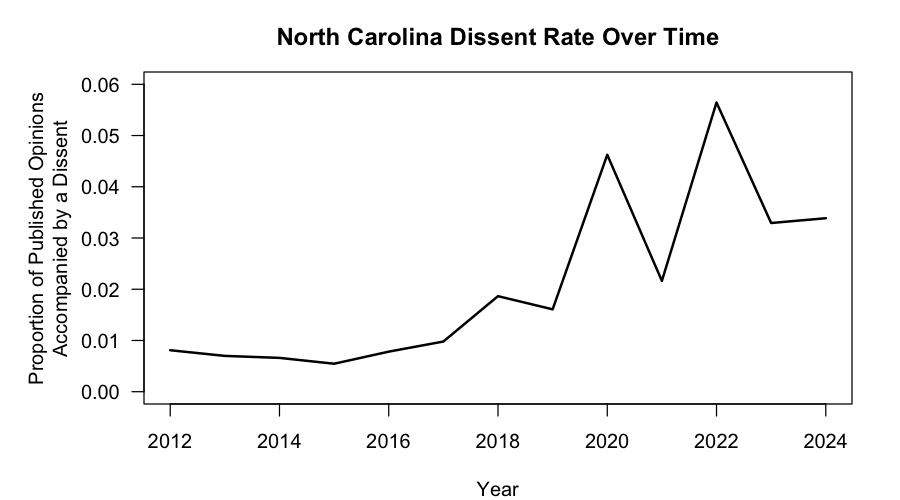
\includegraphics[keepaspectratio,alt={Dissent Rates in North Carolina Supreme Court }]{figures/nc_dissent_rate.png}}
\caption{Dissent Rates in North Carolina Supreme Court
\label{dissent_rates}}
\end{figure}

This section presents the results of the synthetic control analysis. As
shown in \ref{dissent_rates}, North Carolina's dissent rate remained
consistently low (around 1\%) from 2012 to 2017, rising to 1.9\% in 2018
and 4.5\% in 2020, before declining to 2.2\% in 2021 amid
COVID-19-related court closures. Donor courts exhibited more variable
patterns.\footnote{Wisconsin had the highest dissent rates, often
  exceeding 50\% and reaching 88\% in 2016; in many cases, opinion text
  was unavailable, producing fewer results when using Lexis's OpinionBy
  function and likely inflating calculated rates. Arkansas showed
  volatile rates, ranging from 7.7\% in 2012 to over 50\% in 2018--2020.
  Georgia and Minnesota remained relatively stable, typically below
  10\%.}

\begin{figure}
\centering
\pandocbounded{\includegraphics[keepaspectratio,alt={Estimated impact of judicial reform on dissenting behavior }]{figures/scm.png}}
\caption{Estimated impact of judicial reform on dissenting behavior
\label{scm}}
\end{figure}

As shown in \ref{scm}, the synthetic control analysis estimates a
treatment effect of 0.000\%, indicating no detectable change in dissent
behavior following North Carolina's adoption of partisan judicial
elections in 2018. This finding diverges from Renberg's,\footnote{Renberg,
  {``The {Impact} of {Retention Systems} on {Judicial Behavior}.''}} who
finds that switching away from partisan elections is associated with
increased dissent rates, which she attributes to justices being
liberated from electoral constraints and able to assert their legal
philosophy more freely. The present analysis examining the reverse
transition fails to detect an inverse effect when partisan elections are
adopted. One sensitivity analysis provides tentative support for the
null result. Placebo tests that reassign the treatment year to each
pre-intervention year (2014--2017) produce systematic gaps between North
Carolina and its synthetic counterpart. Estimated placebo effects range
from −2.62\% to −3.78\%, with a mean of −2.92\%. The observed 2018
treatment effect of 0.00\% is distinguishable from this placebo
distribution at conventional significance levels (p = 0.042), suggesting
the post-reform period is not simply reflecting pre-treatment variation.
This result should nevertheless be interpreted cautiously. The sections
that follow assess the robustness and substantive credibility of this
null finding in greater detail.

\subsubsection{Model Fit and Pretreatment Covariate
Balance}\label{model-fit-and-pretreatment-covariate-balance}

Mean Squared Prediction Error (MSPE) serves as the principal diagnostic
for assessing the validity of the synthetic control design. Formally,
MSPE is defined as the average squared difference between North
Carolina's observed dissent rates and those predicted by its synthetic
counterpart. Substantively, it measures how closely the synthetic court
reproduces the treated court's pre-intervention trajectory. A low
pre-treatment MSPE is necessary for credible inference, as it indicates
that the synthetic unit approximates a plausible counterfactual prior to
reform. Under those conditions, any subsequent divergence can reasonably
be attributed to the institutional change rather than to model
misspecification.

In the present analysis, the pre-treatment MSPE for 2012-2017 (0.0007)
is consistent with the null hypothesis. At first glance, this small
value appears to indicate strong fit between the synthetic and actual
North Carolina Supreme Court. However, as discussed prior, dissent rates
on the Court are extremely low and display limited variation. In such
sparse data contexts, small absolute MSPE values may simply reflect the
scale of the outcome variable rather than meaningful alignment or
lackthereof in trajectory. Figure \ref{scm} reinforces this finding,
visually illustrating that the synthetic court does not closely track
the North Carolina Supreme Court's actual dissent rates prior to reform.
Additionally, we would expect an increase in the post-treatment MSPE if
partisan elections had altered dissent behavior post-treatment,
reflecting greater divergence between the treated court and its
synthetic counterfactual. Instead, the post-treatment MSPE for
2018--2024 declines to 0.0002. The resulting post-to-pre MSPE ratio of
0.29, well below 1, indicates that model fit actually improves after the
reform. Taken together, this pattern provides little evidence that the
adoption of partisan elections measurably affected dissent rates on the
North Carolina Supreme Court.

A second limitation concerns the distribution of donor weights. The
synthetic control algorithm assigns 100 percent of the donor pool weight
to Minnesota. This eliminates one of SCM's core advantages, as the
algorithm constructs a counterfactual as a weighted composite of
multiple comparison units. Although it is not uncommon for SCM to
allocate weight unevenly across donors, or to exclude some entirely,
such concentration is substantively reassuring only when the selected
unit closely matches the treated unit on pre-treatment characteristics.
This condition is not met in the present study. The full weight placed
on Minnesota does not signal that its supreme court provides a strong
predictive match for North Carolina. Rather, it reflects the algorithm's
constrained optimization under conditions of poor pretreatment balance.

The court serving as the sole contributor to the counterfactual bears
limited structural resemblance to the treated court across several
dimensions. As Table \ref{tab:covariate_balance} shows, 11 of 14
covariates exceed the conventional 0.25 standardized difference
threshold, indicating substantial imbalance. The discrepancies are
especially pronounced in campaign finance (\$1.35 million versus
\$177,336), criminal procedure dockets (0.458 versus 0.129), capital
appeals (0.167 versus 0.333), and electoral competition (0.667 versus
0.000). These differences suggest that, despite receiving full weight in
constructing the synthetic North Carolina Supreme Court, Minnesota's
institutional and political context diverges meaningfully from North
Carolina's prior to reform. This limitation is not unique to the present
study. Although Renberg does not explicitly discuss it, her synthetic
control model shows similar imbalances, including substantial
overestimation of published opinions (by 92--494 percent),
underestimation of criminal procedure dockets by roughly 50 percent in
Arkansas and Mississippi, and pronounced divergences in capital
punishment caseloads.\footnote{Renberg, {``The {Impact} of {Retention
  Systems} on {Judicial Behavior}.''}}

This poor covariate balance may stem from the inherent homogeneity of
state supreme courts, which violates the fundamental parallel trends
assumption of SCM. North Carolina's Supreme Court is structurally
unique: it can bypass the Court of Appeals and holds direct appellate
jurisdiction over constitutional questions, statutory challenges, and
other high-stakes matters. This structure generates a substantially
higher volume of published opinions, which drives down dissent rates.
Additionally, diverse responses to COVID-19 beginning in 2020, including
closures, delayed proceedings, and shifts in case composition, may
further complicate the analysis of dissent rates during the study
period. This suggests that SCM may not be a robust method for studying
dissent rates, and raises questions about the validity of Renberg's
conclusions regarding the impact of selection mechanisms on dissent
behavior and judicial independence.

\begin{table}[p]
\captionsetup{justification=raggedright, singlelinecheck=false, skip=5pt}
\caption{Covariate Balance Between Treated and Synthetic North Carolina}
\label{tab:covariate_balance}
\centering
\begin{tabular}{lccc}
\hline
\rule{0pt}{3ex}\textbf{Covariate}
& \textbf{Treated (NC)}
& \textbf{Synthetic NC}
& \textbf{Sample Mean} \\[1ex]
\hline
Campaign Finance        & 1,348,421 & 177,336 & 381,739 \\
Court Professionalization & 0.609 & 0.610 & 0.612 \\
Capital Appeals         & 0.167 & 0.333 & 2.548 \\
Lower Court Capital Appeals & 1.000 & 0.500 & 1.548 \\
Criminal Procedure Docket & 0.458 & 0.129 & 0.519 \\
Ideological Spread      & 2.283 & 1.964 & 1.291 \\
Citizen Ideology        & 3.903 & 4.161 & 3.933 \\
Government Ideology     & 0.240 & -0.093 & 0.147 \\
Term Length             & 8.000 & 6.000 & 7.429 \\
Number of Justices      & 7.000 & 7.000 & 7.286 \\
Election Structure      & 0.000 & 0.000 & 0.143 \\
Electoral Competition   & 0.667 & 0.000 & 0.167 \\
Published Opinions      & 1,057 & 657 & 224 \\
\hline
\end{tabular}
\end{table}

Moreover, additional sensitivity tests including leave-one-out, placebo,
and year-by-year analyses further illuminate the fragility of causal
inference in this setting. Conducted by systematically excluding each
donor court one at a time and recalculating the treatment effect, the
leave-one-out analysis undermines confidence in the results. A robust
causal estimate should remain stable across reasonable variations in
model specification. By contrast, excluding each donor state supreme
court produces treatment effects ranging from -0.1887 (Minnesota
excluded) to -0.0875 (Wisconsin excluded), with a mean of -0.1617 and
standard deviation of 0.0382. Each leave-one-out specification produces
a negative treatment effect, yet the optimal weighted combination yields
exactly zero. This pattern indicates that the zero treatment effect is
an artifact of the specific weighting scheme rather than a robust
finding.

Additionally, comparing optimal synthetic control weights decided by the
algorithm to artifically equalized weights reveals no difference in
results. Both methods produce an estimated average treatment effect
(ATE) of 0.00, indicating no mean difference in dissent rates between
North Carolina and the synthetic control across all post-treatment
years. This equivalence suggests that the sophisticated weighting
algorithm provides no advantage over a simple average of control courts,
indicating that no weighting scheme can adequately address the severe
covariate imbalances.

Lastly, examining year-by-year treatment effects reveals substantial
temporal instability. The estimated effect of partisan elections on
dissent rates varies dramatically across post-treatment years: 2018
(-0.0123), 2019 (-0.0150), 2020 (+0.0068), 2021 (-0.0005), 2022
(+0.0270), 2023 (-0.0135), 2024 (+0.0078). These estimates range from
-0.015 to +0.027 with a standard deviation of 0.0152, nearly as large as
the effects themselves. If partisan elections truly increased dissenting
behavior through electoral accountability mechanisms, we would expect a
sustained, consistent effect following the 2018 reform. Instead, the
effects fluctuate in both direction and magnitude across years,
suggesting that any apparent treatment effects likely reflect random
variation or temporary fluctuations. Additionally, COVID-19 disruptions
may have introduced temporal shocks that affect the analysis
independently of electoral reform.

Altogether, the poorly fitted MSPE, lopsided weighting of donor courts,
pretreatment imbalances, and failed sensitivity tests highlight
important limitations in using SCM to assess the causal impact of
electoral reform on dissenting behavior. The pre- and post-treatment
MSPE values indicate that the synthetic control provides only a weak
approximation of North Carolina's dissent trajectory. The synthetic
control relies entirely on Minnesota, which bears limited structural
resemblance to North Carolina. Leave-one-out sensitivity tests and
comparisons with equalized donor weights show that the estimated
treatment effect is highly sensitive to the specific donor combination.
Year-by-year estimates further demonstrate substantial temporal
instability. While the pretreatment placebo tests suggest that the zero
treatment effect in 2018 is significantly distinguishable from other
years during the pre-treatment period, this result must be interpreted
cautiously given the scarcity of comparable control units, low-variance
outcomes, substantial covariate imbalances, and hypothesized treatment
effects that are small relative to secular trends and measurement
variability. Collectively, these findings highlight the limitations of
SCM in this context and the broader challenges of studying dissent rates
in highly heterogeneous state supreme court systems.

\subsubsection{Textual Analysis}\label{textual-analysis}

Beyond the constraints already discussed, dissent rates alone provide
only a limited perspective on how electoral reform shapes judicial
behavior. While the prevalence of dissent indicates whether justices
disagree with the majority, it does not reveal the depth, substance, or
reasoning underlying those disagreements. Accordingly, this section
presents a computational textual analysis of judicial dissents, enabling
an assessment of how electoral reform influences the substantive content
of judicial reasoning. In particular, the analysis examines how
different election mechanisms affect both the political and legal tenor
of justices' dissents.

\subsubsection{Wordscores Seed
Dictionaries}\label{wordscores-seed-dictionaries}

\begin{figure}
\centering
\pandocbounded{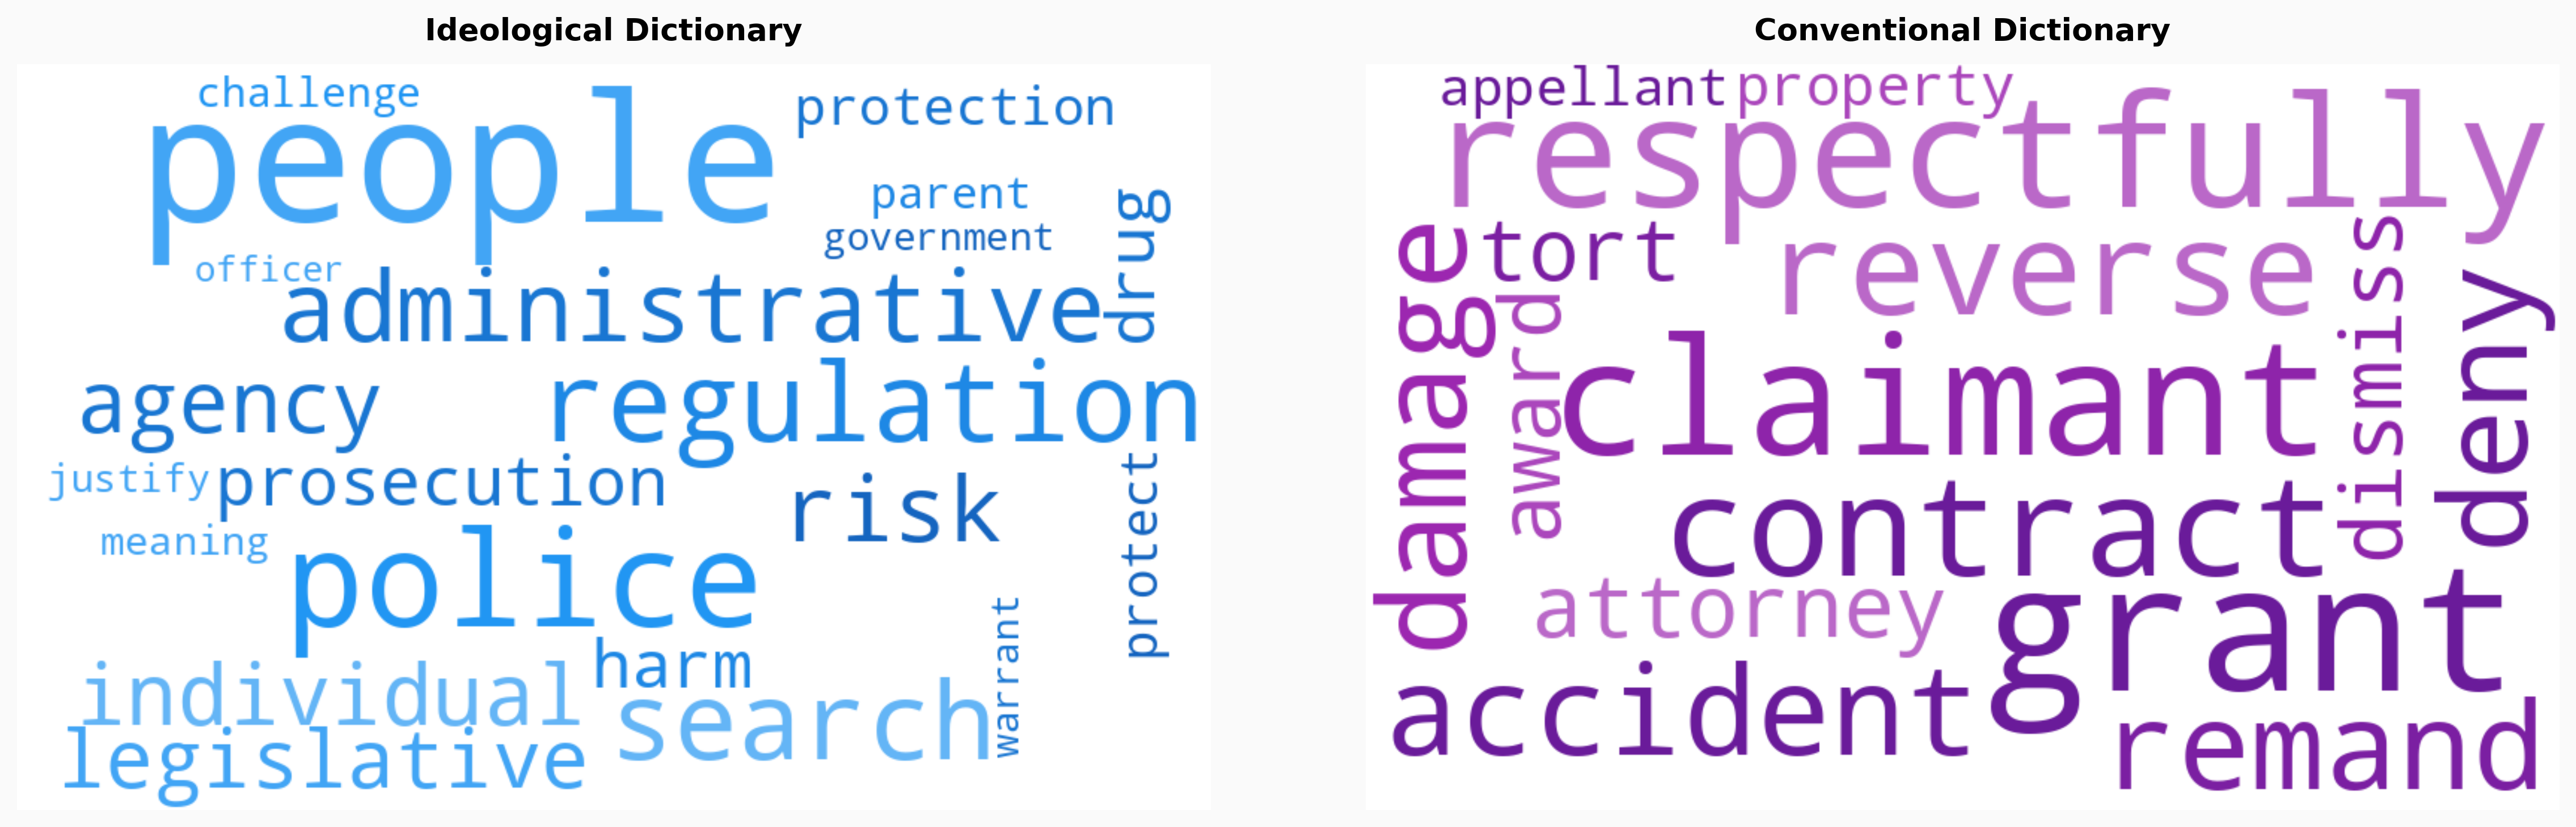
\includegraphics[keepaspectratio,alt={Seed word dictionaries (font size proportional to difference scores) }]{figures/seed_wordclouds.png}}
\caption{Seed word dictionaries (font size proportional to difference
scores) \label{wordclouds}}
\end{figure}

The resulting seed terms shown in \ref{wordclouds}. Both dictionaries
were manually reviewed, and a small number of generic terms or words
reflecting parsing errors were excluded. Words in the ideological
dictionary reflect the tendency of justices with extreme PAJID scores to
engage with constitutional issues and contested legal domains. Terms
such as \emph{search, warrant, police,} and \emph{prosecution} reflect
Fourth Amendment framing and the exercise of state power;
\emph{regulation, legislative, administrative,} and \emph{agency}
characterize debates over the scope of government authority; and
\emph{drug, harm,} and \emph{parent} mark substantively contested
criminal and family law domains shaped by ideological priors. Framing
terms like \emph{individual, government, people, protect, justify,} and
\emph{risk} indicate whom the law serves and on what grounds, while
\emph{meaning} and \emph{challenge} reflect interpretive and adversarial
reasoning. In contrast, the conventional dictionary reflects the
tendency of justices with more centrist PAJID scores to focus on civil
matters while emphasizing collegiality and procedural deference.
Commercial and civil law terms such as \emph{contract, tort, accident,
damage, award,} and \emph{property} anchor opinions in technically
oriented domains of lower ideological salience. Dispositional vocabulary
including \emph{reverse, remand, dismiss, deny,} and \emph{grant}
reflects procedural resolution rather than substantive constitutional
engagement, and collegial terms such as \emph{respectfully} signal
deference to institutional norms. Party and role terms including
\emph{claimant, appellant,} and \emph{attorney} further reinforce the
conventional dictionary's orientation toward procedural rather than
ideological reasoning.

\subsubsection{Word2Vec Dictionary
Expansion}\label{word2vec-dictionary-expansion}

\begin{figure}
\centering
\pandocbounded{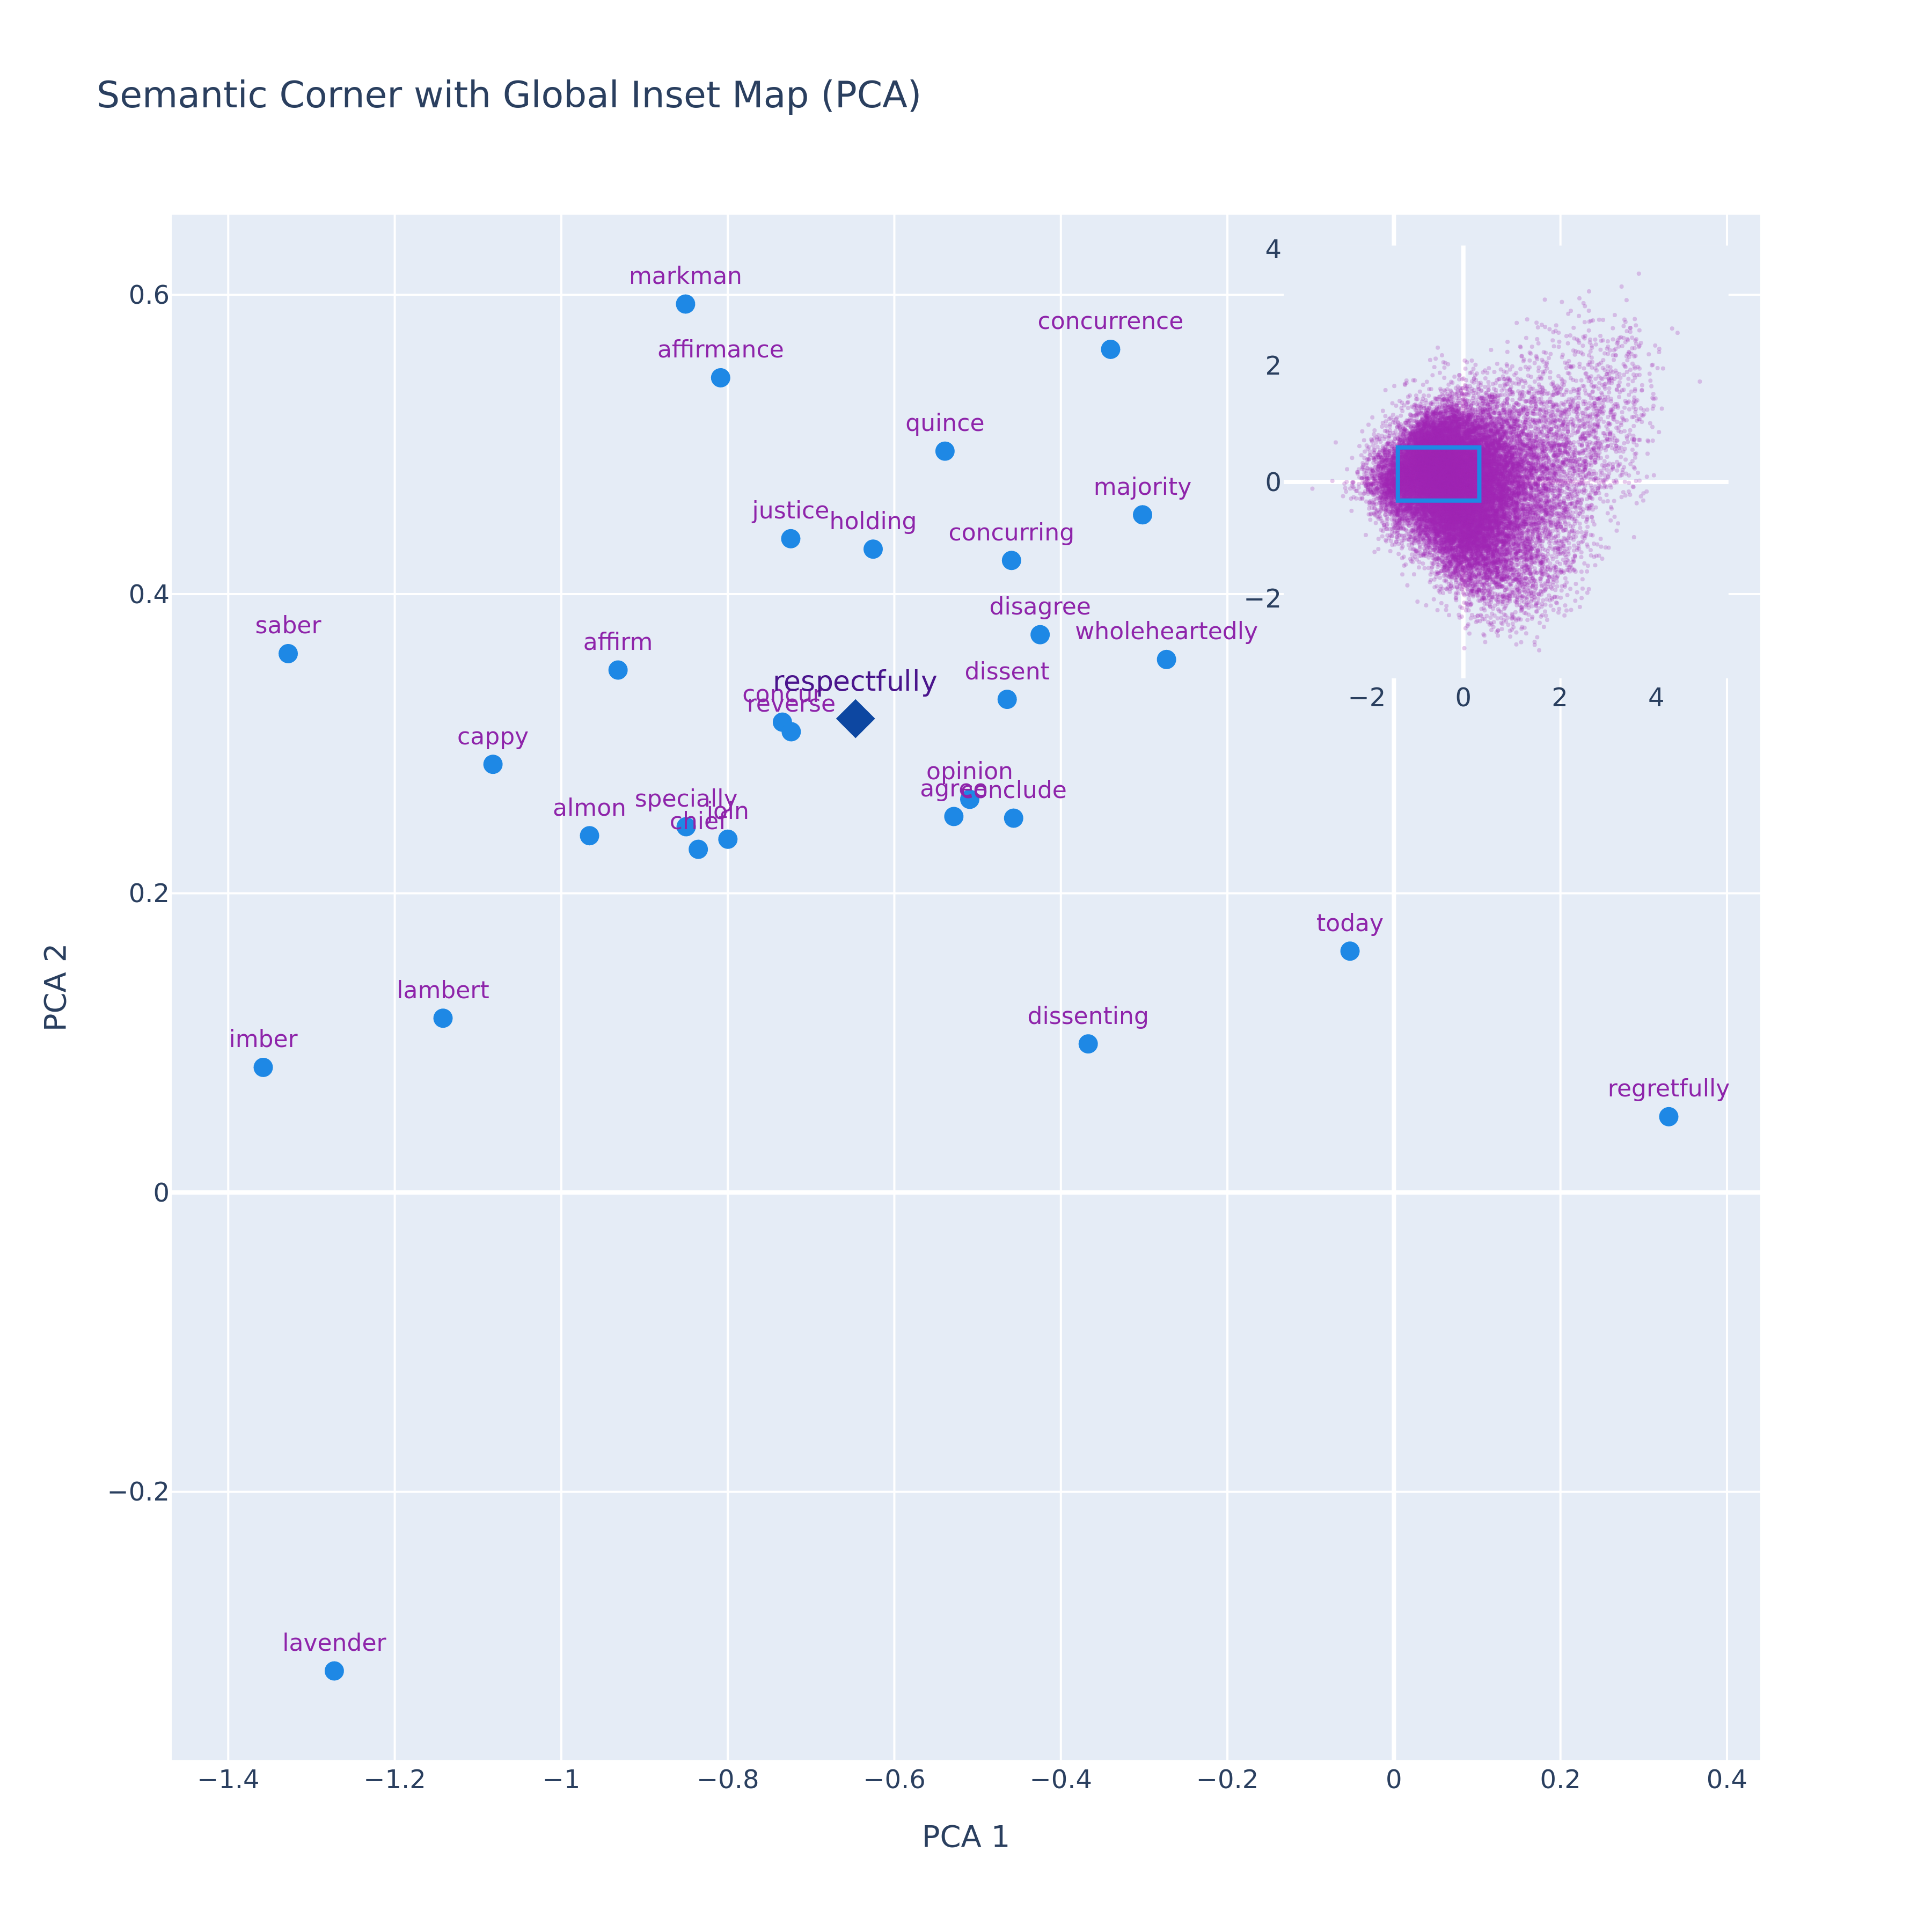
\includegraphics[keepaspectratio,alt={Semantic space around ``respectfully''}]{figures/semantic_corner_plot.png}}
\caption{Semantic space around ``respectfully''\label{semantic_corner}}
\end{figure}

The seed dictionaries were expanded using Word2Vec to compute cosine
similarity between a seed word's vector and all other word vectors in
the embedding space, adding semantically related terms that Wordscores
may have missed due to insufficient frequency in the reference corpora.
\ref{semantic_corner} visualizes the 30 words most semantically similar
to a conventional seed word, \emph{respectfully}, projected into
two-dimensional space using Principal Component Analysis (PCA). The
cluster reveals that \emph{respectfully} associates primarily with
procedural and collegial terminology, \emph{dissent, concur, dissenting,
concurring, affirm, majority, disagree, join, colleague,} and
\emph{reverse.} The inset map (top right) situates this semantic cluster
within the full embedding space of all words in the model, illustrating
how the Word2Vec model captures the contextual meaning of associated
words.

\subsubsection{Rhetoric Scores Results}\label{rhetoric-scores-results}

To assess whether judicial rhetoric has shifted over time, a panel OLS
regression of annual mean rhetoric scores on year was estimated
separately for each selection mechanism, with state fixed effects and
standard errors clustered by state. The overall trend is negligible and
statistically insignificant (\(\beta\) = -0.0004, \(p\) = 0.110),
indicating no secular drift in rhetoric across the full sample once
state-level heterogeneity is accounted for. Within-mechanism trends are
similarly flat: partisan (\(\beta\) = 0.0005, \(p\) = 0.872),
nonpartisan (\(\beta\) = -0.0013, \(p\) = 0.414), and appointment
(\(\beta\) = 0.0004, \(p\) = 0.852) courts show no detectable rhetorical
trend over time. The sole exception is retention election courts, which
exhibit a statistically significant negative trend (\(\beta\) = -0.0037,
\(p\) = 0.017), indicating a modest drift toward more ideological
rhetoric over time among courts using retention elections.

\subsubsection{Level Differences by Selection
Mechanism}\label{level-differences-by-selection-mechanism}

\begin{figure}
\centering
\pandocbounded{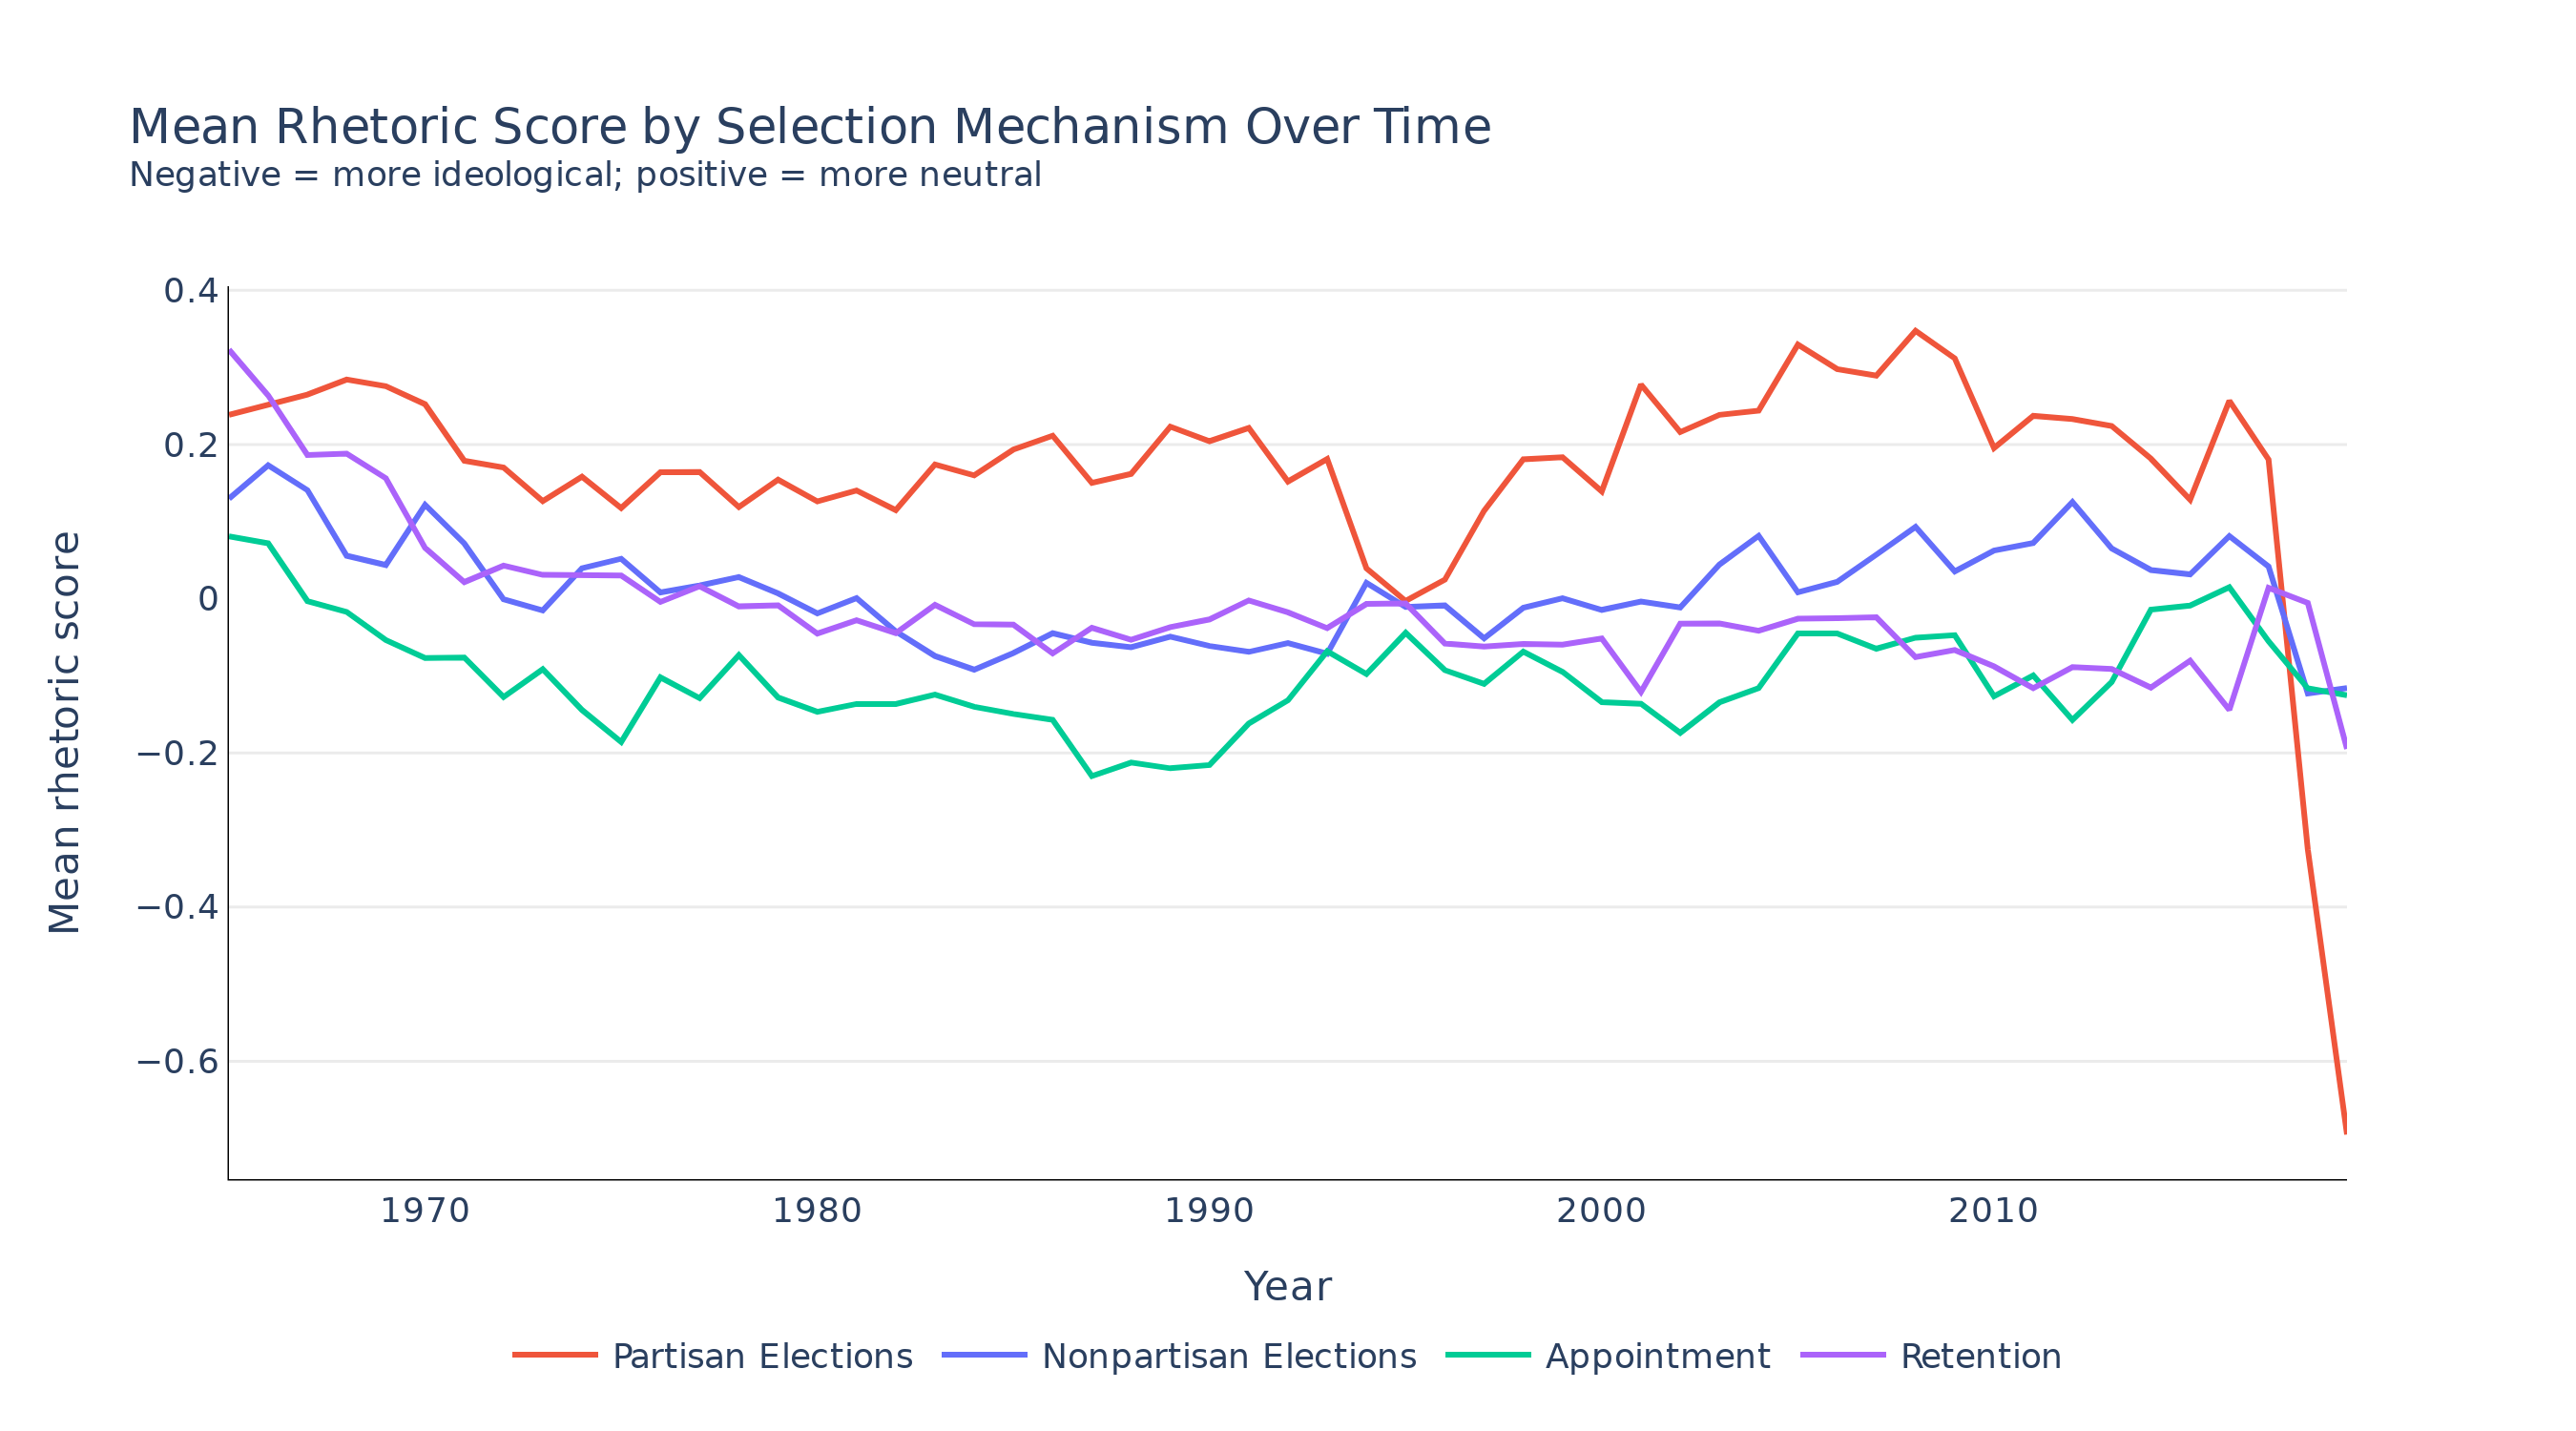
\includegraphics[keepaspectratio,alt={Rhetoric scores over time by selection mechanism}]{figures/rhetoric_by_mechanism.png}}
\caption{Rhetoric scores over time by selection mechanism}
\end{figure}

To assess whether selection mechanisms predict rhetoric levels, a panel
OLS regression of annual mean raw rhetoric scores on mechanism dummies
was estimated with state fixed effects, a linear year control, and
standard errors clustered by state. The analysis is restricted to the
eleven states that switched mechanisms at least once during the study
period, as these are the only states for which within-state variation in
mechanism can identify level effects net of time-invariant court
characteristics. Nonpartisan elections serve as the reference category.

The unadjusted raw means suggest that elected courts write more
conventionally than appointed courts. Counterintuitively, partisan
courts produce the most conventional rhetoric (mean = 0.141), followed
by nonpartisan courts (0.009), retention courts (-0.069), and
appointment courts (-0.116). Once state fixed effects are included, the
pattern reverses and strengthens considerably. Appointment courts
produce significantly more ideological rhetoric than nonpartisan courts
(\(\beta\) = -0.286, SE = 0.056, \(t\) = -5.12, \(p\) \textless{}
0.001), as do retention courts (\(\beta\) = -0.199, SE = 0.050, \(t\) =
-3.95, \(p\) \textless{} 0.001). Partisan election courts trend toward
more conventional rhetoric relative to nonpartisan courts (\(\beta\) =
0.109, SE = 0.059, \(t\) = 1.84, \(p\) = 0.066), though this result
falls just short of conventional significance thresholds. These findings
suggest that the meaningful institutional divide in judicial rhetoric
runs between courts insulated from electoral pressure and those subject
to any form of electoral accountability, rather than between partisan
and nonpartisan systems specifically.

\subsubsection{Event Study: Selection Mechanism
Switches}\label{event-study-selection-mechanism-switches}

To examine the rhetorical consequences of mechanism changes more
directly, a pre/post comparison examines detrended rhetoric scores in
the six years before and after each of the twelve selection mechanism
switches occurring among the 50 courts between 1965 and 2019. A
two-sample \(t\)-test assesses whether the post-switch mean differs
significantly from the pre-switch mean within a \(\pm\) 6 year window
around each switch.

The clearest individual result is Florida's 1971 transition from
partisan to retention elections (\(\Delta\) = -0.264, \(p\) = 0.029),
which produced a statistically significant shift toward more ideological
rhetoric following the removal of contested partisan competition.
Arizona's 1974 transition from nonpartisan to retention elections shows
a similar directional pattern (\(\Delta\) = -0.269, \(p\) = 0.087), as
does Utah's 1985 transition (\(\Delta\) = -0.163, \(p\) = 0.052). Among
all seven transitions toward retention elections, six of seven produce
negative differences, indicating more ideological rhetoric post-switch,
with a mean difference of -0.122. A sign test finds this pattern
marginally consistent with a systematic effect (\(p\) = 0.125), though
the small sample limits power.

Among the four states transitioning from partisan to nonpartisan
elections, including Kentucky, Mississippi, West Virginia, and North
Carolina 2002, three of four produce negative differences, with a mean
of -0.077, though none individually reach significance. Vermont's 1974
appointment-to-retention transition moves in the opposite direction
(\(\Delta\) = +0.358), though this result is not statistically
significant (\(p\) = 0.464).

North Carolina provides the closest available natural experiment, having
switched selection systems twice in opposite directions. The 2002 switch
away from partisan elections was followed by more ideological rhetoric
(\(\Delta\) = -0.150), while the 2018 reinstatement of partisan
elections was also followed by more ideological rhetoric (\(\Delta\) =
-0.097), though neither result reaches significance. The absence of a
mirror-image pattern across both North Carolina switches is inconsistent
with a simple partisan-label effect and reinforces the panel
regression's null finding for the partisan versus nonpartisan
comparison.

Taken together, the panel and event study results point toward a
consistent conclusion. The statistically robust finding is that
electoral accountability in any form --- including mild retention
elections --- is associated with more conventional judicial rhetoric
relative to appointment, once between-state differences are controlled.
The partisan versus nonpartisan distinction, which motivates current
reform debates, does not produce a detectable or consistent rhetorical
difference in either the panel regression or individual event studies.
These findings suggest that the institutional divide that matters most
for judicial rhetoric runs between insulated and electorally accountable
courts, rather than between partisan and nonpartisan electoral systems
specifically.

Potentially, selection mechanisms may not change the way justices write
because they do not have to do any signalling in their opinions at all.
The party heuristic may be stronger than all else.

\subsection{Conclusion}\label{conclusion}

Conclusion

\newpage

\subsection{References}\label{references}

\newpage

\subsection{Appendix}\label{appendix}

\begin{landscape}
\begin{table}[p]
\centering
\caption{Comparison of Dissent Rate Measurement Methods Across Courts (1995-2010)}
\label{tab:dissent_rates_replication}
\begin{tabular}{l*{9}{r}rrrrrrrrrrrrrrrrrr}
& \multicolumn{3}{c}{\textbf{Hall \& Windett (2013)}} & \multicolumn{3}{c}{\textbf{OpinionBy \& DissentBy}} & \multicolumn{3}{c}{\textbf{AND NOT Method}} \\
\cmidrule(lr){2-4} \cmidrule(lr){5-7} \cmidrule(lr){8-10}
\textbf{Court} & Opinions & Dissents & Rate & Opinions & Dissents & Rate & Opinions & Dissents & Rate \\
\midrule
NC & 13,241 & 154 & 0.0116 & 15,660 & 159 & 0.0102 & 10,687 & 156 & 0.0146 \\
OR & 1,155 & 143 & 0.1238 & 1,074 & 325 & 0.3026 & 331 & 91 & 0.2749 \\
WV & 2,218 & 765 & 0.3449 & 1,253 & 678 & 0.5411 & 351 & 163 & 0.4644 \\
MO & 1,874 & 267 & 0.1425 & 3,271 & 533 & 0.1629 & 484 & 75 & 0.1550 \\
MA & 2,808 & 172 & 0.0613 & 2,731 & 534 & 0.1955 & 780 & 152 & 0.1949 \\
ME & 3,233 & 227 & 0.0702 & 2,464 & 408 & 0.1656 & 1,002 & 136 & 0.1357 \\
IL & 2,302 & 616 & 0.2676 & 1,685 & 630 & 0.3739 & 399 & 141 & 0.3534 \\
ID & 2,119 & 244 & 0.1151 & 2,141 & 439 & 0.2050 & 551 & 110 & 0.1996 \\
HI & 2,086 & 282 & 0.1352 & 1,768 & 389 & 0.2200 & 661 & 86 & 0.1301 \\
AZ & 1,546 & 167 & 0.1080 & 2,802 & 241 & 0.0860 & 336 & 39 & 0.1161 \\
AK & 2,506 & 272 & 0.1085 & 1,923 & 269 & 0.1399 & 543 & 66 & 0.1215 \\
AL & 5,185 & 1,423 & 0.2744 & 4,474 & 1,418 & 0.3169 & 1,626 & 563 & 0.3462 \\
\bottomrule
\end{tabular}
\end{table}
\end{landscape}

\protect\phantomsection\label{refs}
\begin{CSLReferences}{1}{1}
\bibitem[\citeproctext]{ref-Abadie2010}
Abadie, Alberto, Alexis Diamond, and Jens Hainmueller. {``Synthetic
{Control Methods} for {Comparative Case Studies}: {Estimating} the
{Effect} of {California}'s {Tobacco Control Program}.''} \emph{Journal
of the American Statistical Association} 105, no. 490 (2010): 493--505.
\url{https://doi.org/10.1198/jasa.2009.ap08746}.

\bibitem[\citeproctext]{ref-Abadie2003}
Abadie, Alberto, and Javier Gardeazabal. {``The {Economic Costs} of
{Conflict}: {A Case Study} of the {Basque Country}.''} \emph{American
Economic Review} 93, no. 1 (2003): 113--32.
\url{https://doi.org/10.1257/000282803321455188}.

\bibitem[\citeproctext]{ref-Aroyehun2025}
Aroyehun, Segun T., Almog Simchon, Fabio Carrella, Jana Lasser, Stephan
Lewandowsky, and David Garcia. {``Computational Analysis of {US}
Congressional Speeches Reveals a Shift from Evidence to Intuition.''}
\emph{Nature Human Behaviour} 9, no. 6 (2025): 1122--33.
\url{https://doi.org/10.1038/s41562-025-02136-2}.

\bibitem[\citeproctext]{ref-Berry2010}
Berry, William D., Richard C. Fording, Evan J. Ringquist, Russell L.
Hanson, and Carl E. Klarner. {``Measuring {Citizen} and {Government
Ideology} in the {U}.{S}. {States}: {A Re-appraisal}.''} \emph{State
Politics \& Policy Quarterly} 10, no. 2 (2010): 117--35.
\url{https://www.jstor.org/stable/27867139}.

\bibitem[\citeproctext]{ref-Berry1998}
Berry, William D., Evan J. Ringquist, Richard C. Fording, and Russell L.
Hanson. {``Measuring {Citizen} and {Government Ideology} in the
{American States}, 1960-93.''} \emph{American Journal of Political
Science} 42, no. 1 (1998): 327--48.
\url{https://doi.org/10.2307/2991759}.

\bibitem[\citeproctext]{ref-Brace1990}
Brace, Paul, and Melinda Gann Hall. {``Neo-{Institutionalism} and
{Dissent} in {State Supreme Courts}.''} \emph{The Journal of Politics}
52, no. 1 (1990): 54--70. \url{https://doi.org/10.2307/2131419}.

\bibitem[\citeproctext]{ref-StateSupremeCourtProject}
---------. \emph{State {Supreme Court Data Project}}. n.d. Accessed
February 22, 2026.
\href{https://www.ruf.rice.edu//textasciitilde\%20pbrace/statecourt/}{https://www.ruf.rice.edu/\textbackslash textasciitilde
pbrace/statecourt/}.

\bibitem[\citeproctext]{ref-BraceLangerHall2000}
Brace, Paul, Laura Langer, and Melinda Gann Hall. {``Measuring the
{Preferences} of {State Supreme Court Judges}.''} \emph{The Journal of
Politics} 62, no. 2 (2000): 387--413.
\url{https://doi.org/10.1111/0022-3816.00018}.

\bibitem[\citeproctext]{ref-Canon1970}
Canon, Bradley C., and Dean Jaros. {``External {Variables},
{Institutional Structure} \& {Dissent} on {State Supreme Courts}.''}
\emph{Polity} 3, no. 2 (1970): 175--200.
\url{https://doi.org/10.2307/3233984}.

\bibitem[\citeproctext]{ref-DIME}
\emph{Database on {Ideology}, {Money} in {Politics}, and {Elections}
({DIME}): {Public} Version 4.0 \textbar{} {Stanford Libraries Social
Science Data Collection}}. n.d. Accessed January 17, 2026.
\url{https://data.stanford.edu/dime}.

\bibitem[\citeproctext]{ref-EpsteinLandesPosner2011}
Epstein, Lee, William M. Landes, and Richard A. Posner. {``Why ({And
When}) {Judges Dissent}: {A Theoretical And Empirical Analysis}.''}
\emph{Journal of Legal Analysis} 3, no. 1 (2011): 101--37.
\url{https://doi.org/10.1093/jla/3.1.101}.

\bibitem[\citeproctext]{ref-HallAndWindett2016}
Hall, Matthew E. K., and Jason Harold Windett. {``Discouraging
{Dissent}: {The Chief Judge}'s {Influence} in {State Supreme Courts}.''}
\emph{American Politics Research} 44, no. 4 (2016): 682--709.
\url{https://doi.org/10.1177/1532673X16640743}.

\bibitem[\citeproctext]{ref-HallAndWindett2013}
---------. {``New {Data} on {State Supreme Court Cases}.''} \emph{State
Politics \& Policy Quarterly} 13, no. 4 (2013): 427--45.
\url{https://www.jstor.org/stable/24710959}.

\bibitem[\citeproctext]{ref-Hall2001}
Hall, Melinda Gann. {``State {Supreme Courts} in {American Democracy}:
{Probing} the {Myths} of {Judicial Reform}.''} \emph{The American
Political Science Review} 95, no. 2 (2001): 315--30.
\url{https://www.jstor.org/stable/3118123}.

\bibitem[\citeproctext]{ref-FollowTheMoney}
\emph{Home - {FollowTheMoney}.org}. n.d. Accessed January 17, 2026.
\url{https://www.followthemoney.org/}.

\bibitem[\citeproctext]{ref-Voteview2026}
Lewis, Jeffrey B., Keith Poole, Howard Rosenthal, Adam Boche, Aaron
Rudkin, and Luke Sonnet. {``Voteview: {Congressional Roll-Call Votes
Database}.''} In \emph{Voteview: Congressional Roll-Call Votes
Database}. 2026. \url{https://voteview.com/}.

\bibitem[\citeproctext]{ref-LexisNexis}
\emph{{NexisUni}}. LexisNexis, n.d. Accessed January 17, 2026.
\url{https://advance-lexis-com.turing.library.northwestern.edu/firsttime?crid=151f04a4-41f3-4caa-9fd6-1ad2972659d7}.

\bibitem[\citeproctext]{ref-Renberg2020}
Renberg, Kristen M. {``The {Impact} of {Retention Systems} on {Judicial
Behavior}: A {Synthetic Controls Analysis} of {State Supreme Courts}.''}
\emph{The Justice System Journal} 41, no. 4 (2020): 292--312.
\url{https://www.jstor.org/stable/27224753}.

\bibitem[\citeproctext]{ref-Squire2021}
Squire, Peverill, and Jordan Butcher. {``An {Update} to the {Squire
State Court} of {Last Resort Professionalization Index}.''} \emph{State
Politics \& Policy Quarterly} 21, no. 3 (2021): 326--33.
\url{https://doi.org/10.1017/spq.2020.7}.

\bibitem[\citeproctext]{ref-Ballotpedia}
{``State Supreme Courts.''} In \emph{Ballotpedia}. n.d. Accessed January
17, 2026. \url{https://ballotpedia.org/State/_supreme/_courts}.

\bibitem[\citeproctext]{ref-Montana2025}
Van Kley, Constance. {``The {Montana Legislature}'s {Partisan Attack} on
{Judicial Independence}.''} In \emph{State Court Report}. 2025.
\url{https://statecourtreport.org/our-work/analysis-opinion/montana-legislatures-partisan-attack-judicial-independence}.

\bibitem[\citeproctext]{ref-WilkinsonFAIR2016}
{Wilkinson, Mark D., Michel Dumontier, IJsbrand Jan Aalbersberg, et al.}
{``The {FAIR Guiding Principles} for Scientific Data Management and
Stewardship.''} \emph{Scientific Data} 3, no. 1 (2016): 160018.
\url{https://doi.org/10.1038/sdata.2016.18}.

\end{CSLReferences}
